\documentclass{article}
\usepackage{graphicx}				
\usepackage{mathtools}	
\usepackage{hyperref}

\begin{document}
\title{The error function}
\author{Jedrzej Jawor}
\date{}
\maketitle

\section{Normal distribution}

A random variable Y that is normally distributed over a range in x can be described using a gaussian curve \cite{wikigauss}.
 
A gaussian curve is desctribed by two parameters: the mean and the variance. 

The mean $\mu$, also called the expectation value, is the average value 
of a large sample af Y.

The variance $\sigma^2$ is a measure of the dispersion in the distribution of Y. A distribution with low $\sigma^2$ will be much
more localized than a distribution with high $\sigma^2$.
\\
The formula describing the normal distribution is:
\begin{equation}
\label{eq:norm}
f(x,\mu \sigma^2) = \frac{1}{2 \pi \sigma^2} \exp(- \frac{(x-\mu)^2}{2 \sigma^2}).
\end{equation}
The gaussian curve with different parameters is shown in figure \ref{fig:gauss}. 


\begin{figure}[h]
\label{fig:gauss}
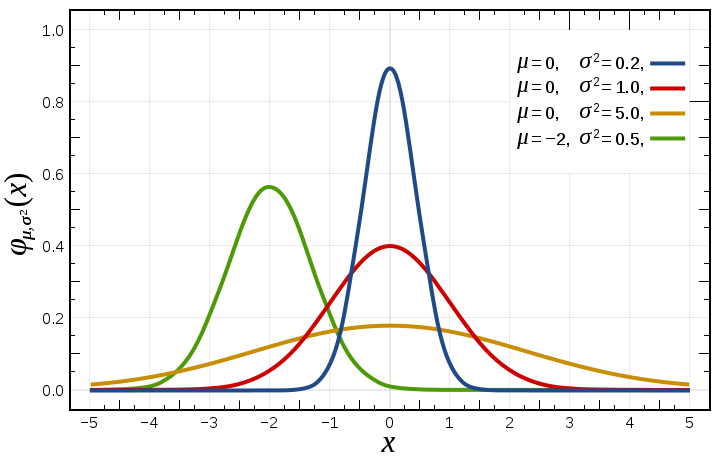
\includegraphics[width=\linewidth]{norm.png}
\caption{Gaussian curves with different values of the mean ($\mu$) and variance ($\sigma^2$)}
\end{figure} 

\section{Error function}
The gaussian curve defined in equation \ref{eq:norm} contains the properties of the normal distribution. In order to extract some of these
properties, auxillary functions, such as the error function, are implemented \cite{wikierf}.
\\
Considering a normally distributed varaible Y with a mean $\mu_Y=1$ and variance $\sigma_Y=1/2$ the errorfunction erf(x) 
will describe the probability of Y falling in the range [-x x].
\\
The error function is defined as:
\begin{equation}
erf(x)=\int_{0}^{x} \frac{2}{\sqrt{\pi}} \exp(-x^2) dx
\end{equation}   
The value of the error function can be evaluated by numerically solving the above integral. The result of this 
evaluation is shown in figure \ref{fig:erf}.

\begin{figure}[h]
\label{fig:erf}
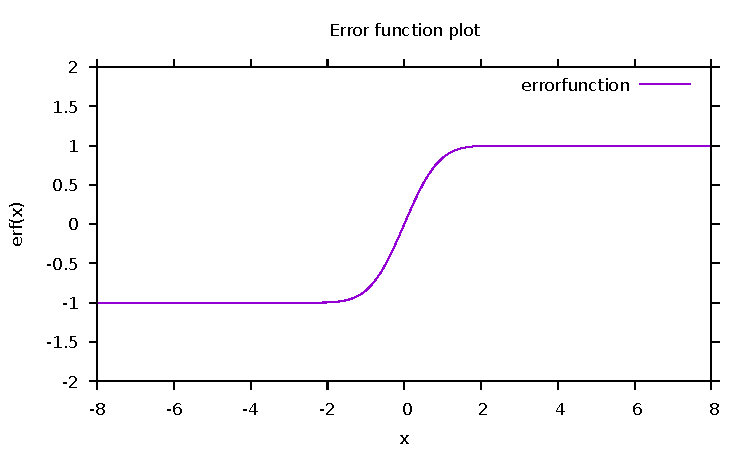
\includegraphics{final.pdf}
\caption{Numerical solution of the error function}
\end{figure}

\clearpage
\section{References}
\begin{thebibliography}{99}
\bibitem{wikigauss}
  Wikipedia article on the gaussian distribution\\
  \emph{WIKIPEDIA: NORMAL DISTRIBUTION},\\
 \url{https://en.wikipedia.org/wiki/Normal_distribution}\\
\\
\bibitem{wikierf}
  Wikipedia article on the error function\\
  \emph{WIKIPEDIA: ERROR FUNCTION},\\
 \url{https://en.wikipedia.org/wiki/Error_function#Applications}\\

\end{thebibliography}

\end{document}
